% begin module optimization-ex1
\abovedisplayskip=0pt
\belowdisplayskip=0pt
\abovedisplayshortskip=0pt
\belowdisplayshortskip=0pt
\begin{frame}
\begin{example}
Find the point on the parabola $y=x^2$ closest to the point $(-20,14)$.
\begin{columns}
\column{2.2in}
\begin{center}
\only<handout:0|1>{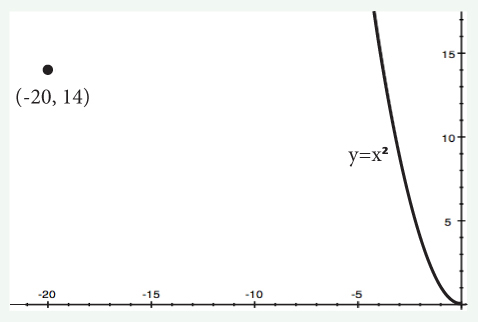
\includegraphics[height=3cm]{optimization/pictures/optimization-ex2a.jpg}}
\only<handout:0|2>{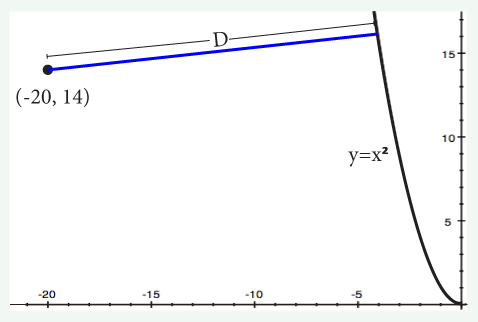
\includegraphics[height=3cm]{optimization/pictures/optimization-ex2b.jpg}}
\only<handout:0|3-18>{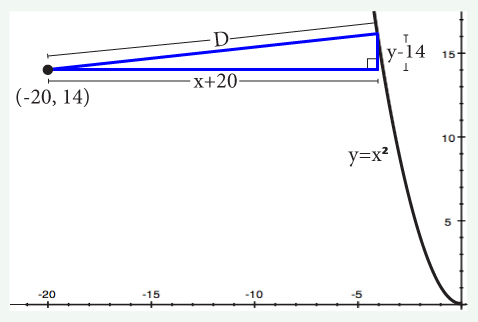
\includegraphics[height=3cm]{optimization/pictures/optimization-ex2c.jpg}}
\only<19>{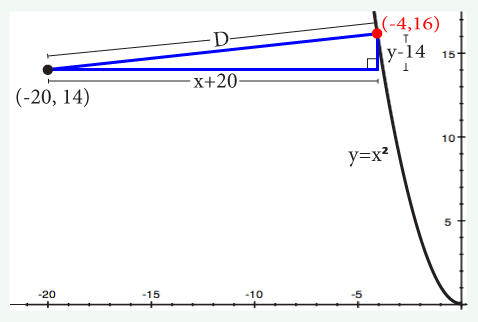
\includegraphics[height=3cm]{optimization/pictures/optimization-ex2d.jpg}}

\uncover<2->{Let $D$ denote the distance from $\alertNoH{4-5}{y=x^2}$ to $(-20,14)$. Then:}
\vspace{3 mm}
\begin{align*}
\uncover<3->{D^2&=(x-(-20))^2+(\alertNoH{4-5}{y}-14)^2}\\
\uncover<4->{&=(x+20)^2+(\alertNoH{4-5}{(\uncover<5->{x^2})}-14)^2}\\
\uncover<6->{&=x^2+40x+400+x^4-28x^2+196}\\
\uncover<7->{&=\alertNoH{9-10}{x^4-27x^2+40x+596.}}
\end{align*}
\end{center}
\column{1.9in}
\begin{center}
\uncover<8->{Find $D'$ and set it equal to zero:}
\begin{align*}
\uncover<9->{\alertNoH{9-12}{\frac{\diff}{\diff x}(D^2)} & \alertNoH{9-10}{ =  \uncover<10->{4x^3-54x+40}}}   \\
 \uncover<11->{\uncover<12->{\alertNoH{12}{2D \cdot \alertNoH{13}{D'}}} &= 4x^3-54x+40} \\
\uncover<13->{2D \cdot \alertNoH{13}{0} &=4x^3-54x+40}\\
\uncover<14->{-40 &=2x(2x^2-27)}\\
\uncover<15->{-20 &=x(2x^2-27)}
\end{align*}

\uncover<16->{Solve by guessing, using divisors of $20$ for $x$.}\\
\uncover<17->{$x =-4$, } \uncover<18->{$y = (-4)^2=16$}\\
\uncover<19->{Closest point is $(-4,16)$.}
\end{center}
\end{columns}
\end{example}
\end{frame}
% end module optimization-ex1
